\begin{frame}
  \titlepage

  \centering
  Alberi evolutivi
\end{frame}



\begin{frame}
\frametitle{Evolution}

\centering
\includegraphics<1>[height=0.6\textheight]{figures/evolution-desk-720x380.jpg}

\begin{itemize}
  \item
    Change over generations
  \item Random mutations
  \end{itemize}
\end{frame}

% \begin{frame}
% \frametitle{Good Evolution}

% \centering
% \includegraphics<1>[height=0.6\textheight]{figures/selective-pressure.jpg}

% \end{frame}

\begin{frame}
\frametitle{Actual Mutation}
 
\centering
\includegraphics<1>[height=0.6\textheight]{figures/dna_strand.jpg}

\end{frame}



\begin{frame}
\frametitle{Hollywood Mutation}

\centering
\includegraphics<1>[height=0.85\textheight]{figures/spiderman-spider-bite-comic}
\end{frame}


\begin{frame}
\frametitle{Individual Evolution}

\centering
  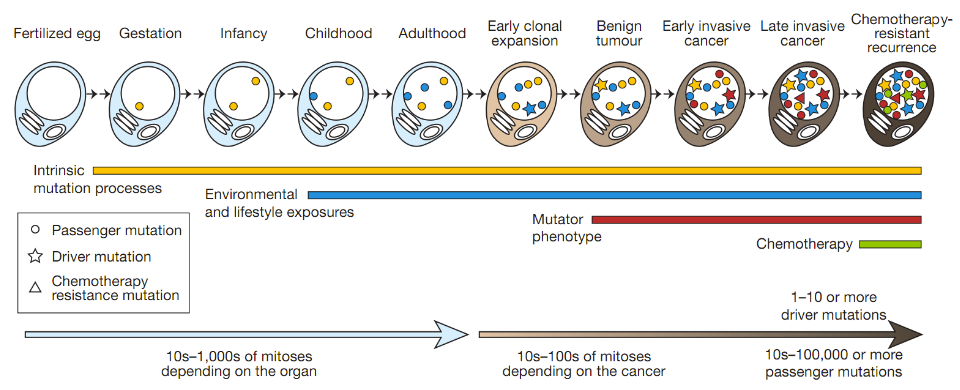
\includegraphics[width=\linewidth]{figures/progression}
  \begin{itemize}
    \item
      Cells \alert{accumulate} mutations throughout the entire life
  % \item
  %   Accumulate mutation $\Rightarrow$ perfect phylogeny
  \end{itemize}
\end{frame}




\begin{frame}
\frametitle{Character-based evolution}

\centering
\includegraphics<1>[height=0.55\textheight]{figures/perfect-phylogeny}

\begin{block}{A possible rule}
Each character is gained \alert{exactly once} in the tree.
\end{block}
\end{frame}


\begin{frame}
  \frametitle{Perfect Phylogeny Problem}
\begin{columns} 
  \begin{column}{0.48\textwidth}
{    \scriptsize
 \begin{tabular}{l|ccccc}
        & A & J & H & L & V\\ \hline
        Scorpion& 0 & 0 & 0 & 0 & 0\\
        Lamprey& 0 & 0 & 0 & 0 & 1\\
        Tuna& 0 & 1 & 0 & 0 & 1\\
        Salamander& 0 & 1 & 0 & 1 & 1\\
        Turtle& 1 & 1 & 0 & 1 & 1\\
        Leopard& 1 & 1 & 1 & 1 & 1
 \end{tabular}
}\begin{block}{Problem}
  \begin{itemize}
    \item
  Input: a binary matrix $M$
    \item
      Output: a tree \alert{explaining} $M$, if it exists
\end{itemize}
\end{block}

\end{column}
    
    \begin{column}{0.48\textwidth}
      \centering
\includegraphics<1>[height=0.52\textheight]{figures/perfect-phylogeny}
\end{column}
\end{columns}
\begin{block}{Linear time algorithm (Gusfield, Networks 1991)}
  \begin{enumerate}
    \item
      Radix Sort the columns by decreasing number of $1$s
    \item
      Build the tree, inserting the species one at a time
    \end{enumerate}
  \end{block}
\end{frame}




% \begin{frame}
% \frametitle{Losing characters}

% \centering
% \includegraphics<1>[height=0.65\textheight]{figures/classification-of-life-taxonomy}

% \begin{block}{A possible rule}
% Each character can be lost (once).
% \end{block}

% \end{frame}




\begin{frame}
\frametitle{Characters and States}

\begin{block}{Change of state}
  \begin{itemize} 
\item  A character $c$ is \alert{gained} $\Rightarrow$  the state of $c$ changes from $0$ to $1$
  in an edge
\item  A character $c$ is \alert{lost} $\Rightarrow$  the state of $c$ changes from $1$ to $0$
  in an edge (\alert{backmutation})
\end{itemize}
\end{block}

\begin{block}{Models of Evolution}
  Each character $c$ is gained \alert{exactly once} in the tree.
\begin{enumerate}
\item
  Perfect Phylogeny:  No backmutations
\item
  Persistent Phylogeny: Each character can be lost at most once in the tree.
\alert{$012$ model}
\item
  \alert{Dollo} parsimony: 
  Unlimited backmutations
\end{enumerate}
\end{block}
\end{frame}



\begin{frame}
\frametitle{Tumors}
\begin{columns}
\begin{column}{0.75\textwidth}
\centering
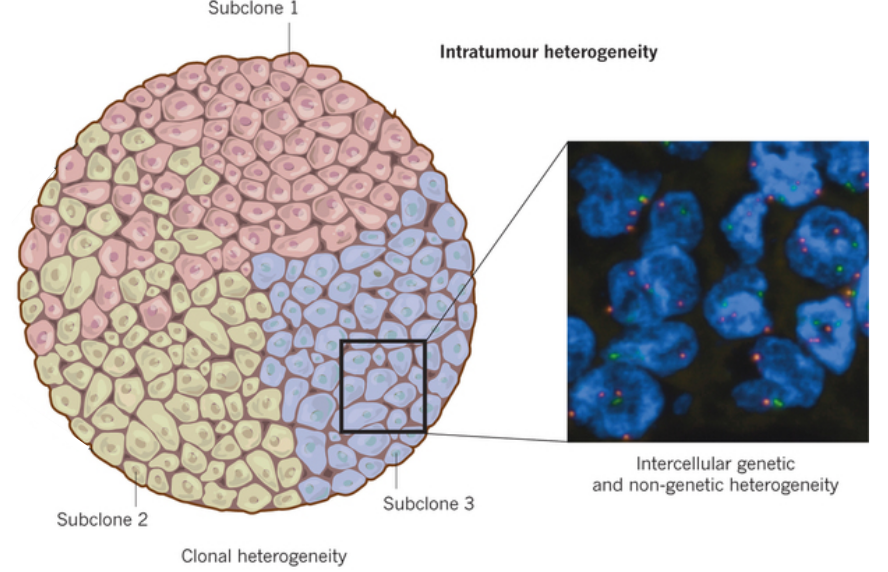
\includegraphics[width=0.9\linewidth]{figures/tumor-heterogeneous}
\end{column}
\begin{column}{0.25\textwidth}
\begin{itemize}
\item
A \alert{tumor} is a mixture of healthy and cancer cells
\item
A \alert{tumor} is a mixture of cancer clones
\end{itemize}
\end{column}
\end{columns}
\end{frame}


\begin{frame}
\frametitle{Tumor Evolution}
\begin{columns}
\begin{column}{0.75\textwidth}
\centering
  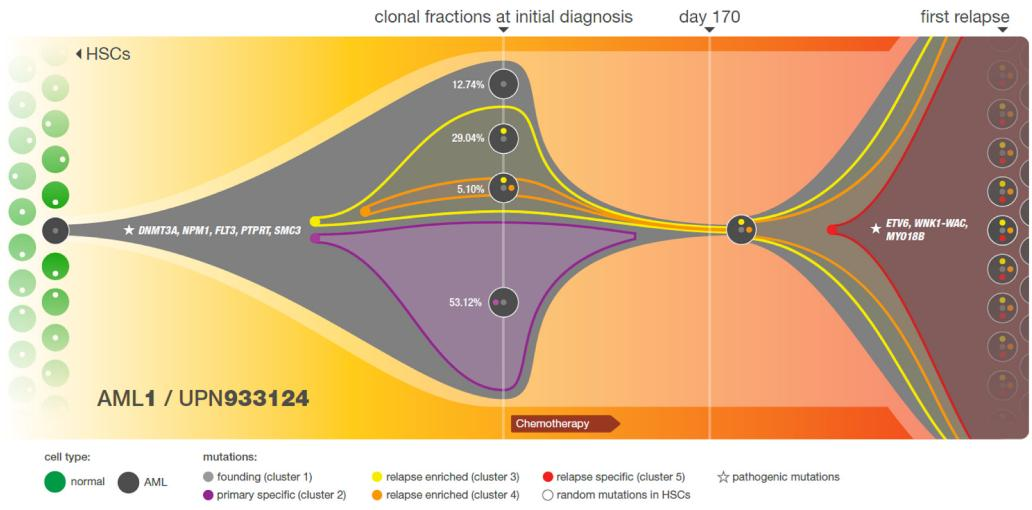
\includegraphics[width=0.99\linewidth]{figures/clonal}
\end{column}
\begin{column}{0.25\textwidth}
\begin{itemize}
\item Different clones make different fractions of the tumor 
\end{itemize}
\end{column}
\end{columns}
\end{frame}


\def\mut#1#2{%
\begin{scope}[shift={#1}]
\node[thick,draw,fill=blue!70,circle, scale=3.5] (#2) {};
\end{scope}
}

\def\muta#1#2{%
\begin{scope}[shift={#1}]
\mut{(0,0)}{#2};
\draw[fill=white] (0,0) circle (.1);
\end{scope}
}

\def\mutb#1#2{%
\begin{scope}[shift={#1}]
\muta{(0,0)}{#2};
\node[fill,color=brown,star, star points=6,scale=0.75] at (45:0.3) {};
\end{scope}
}

\def\mutc#1#2{%
\begin{scope}[shift={#1}]
\muta{(0,0)}{#2};
\node[fill,color=green,regular polygon, regular polygon sides=3,scale=0.65] at (90:0.3) {};
\end{scope}
}

\def\mutd#1#2{%
\begin{scope}[shift={#1}]
\mutc{(0,0)}{#2};
\node[fill,color=red,regular polygon, regular polygon sides=4,scale=0.75] at (0:0.3) {};
\end{scope}
}

\def\mute#1#2{%
\begin{scope}[shift={#1}]
\mutd{(0,0)}{#2};
\node[draw,cross out, draw=pink, very thick,scale=.8] at (180:.3) {};
\end{scope}
}

\def\mutf#1#2{%
\begin{scope}[shift={#1}]
\mutd{(0,0)}{#2};
\node[draw,diamond,scale=0.6, fill,color=blue]  at (270:0.3) {};
\end{scope}
}

\begin{frame}
\frametitle{Tumor Evolution}

\begin{columns} 
  \begin{column}{0.38\textwidth}
\centering
\resizebox{0.95\textwidth}{!}{\begin{tikzpicture}[,>=triangle 60]
\mutf{(-5,5)}{s5};
\muta{(-5.5,7)}{s4};
\muta{(-4,9)}{s4};

\muta{(-2.4,5.8)}{s4};
\mutb{(-1.2,6.7)}{s1};
\mutb{(-3.5,7)}{s1};
\mutc{(-2,8.2)}{s3};
\mutc{(-0.2,8)}{s3};

\mutc{(-4,2)}{s1};
\mut{(-2.5,2)}{};
\mut{(0.5,3.5)}{};
\mut{(-4.5,3.5)}{};
\mutd{(0.5,1.8)}{s6};
\mute{(-3,3.5)}{s2};
\mutf{(-1.2,3)}{s5};
\mutc{(0.5,5)}{s32};

\draw[rotate=30,thick] (2,7) ellipse (2.8 and 2.1);
\node at (-4,0.5) {Sample 1};
\draw[rotate=0,thick] (-3,2.8) ellipse (2.8 and 1.8);
\node at (-2,10) {Sample 2};
\end{tikzpicture}}
\end{column}
  \begin{column}{0.58\textwidth}

\begin{itemize}
\item A \alert{sample} is a mixture of clones
\item For each sample, we have the \alert{frequency} of each mutation
\item
  frequency matrix $F$
%\item inference of tumoral phylogeny
\end{itemize}

\centering
\resizebox{0.95\textwidth}{!}{\begin{tikzpicture}[scale=0.8]
\draw[fill=white] (3,2) circle (.1);
\node[fill,color=brown,star, star points=6,scale=0.75] at (6,2) {};
\node[fill,color=green,regular polygon, regular polygon sides=3,scale=0.65] at (2,2) {};
\node[draw,cross out, draw=pink, very thick,scale=.8] at (5,2) {};
\node[draw,diamond,scale=0.6, fill,color=blue]  at (1,2) {};
\node[fill,color=red,regular polygon, regular polygon sides=4,scale=0.75] at (4,2) {};

\node at (1,1) {0.2}; \node at (2,1) {0.6}; \node at (3,1) {0.6};
\node at (4,1) {0.4}; \node at (5,1) {0.2}; \node at (6,1) {0.0};
\node at (1,0) {0.0}; \node at (2,0) {0.4}; \node at (3,0) {1.0};
\node at (4,0) {0.0}; \node at (5,0) {0.0}; \node at (6,0) {0.4};

\node at (0,1) {$S_{1}$}; \node at (0,0) {$S_{2}$};
\end{tikzpicture}}

\end{column}
\end{columns}
\end{frame}


\begin{frame}
\frametitle{Tumor Evolution: Compute}

\begin{columns} 
  \begin{column}{0.40\textwidth}
    \begin{block}{Matrix $B$ representing tree $T$}
    \end{block}
\centering
\resizebox{0.61\textwidth}{!}{\begin{tikzpicture}[scale=0.44]
\draw[fill=white] (3,2) circle (.1);
\node[fill,color=brown,star, star points=6,scale=0.5] at (6,2) {};
\node[fill,color=green,regular polygon, regular polygon sides=3,scale=0.5] at (2,2) {};
\node[draw,cross out, draw=pink, very thick,scale=.6] at (5,2) {};
\node[draw,diamond,scale=0.46, fill,color=blue]  at (1,2) {};
\node[fill,color=red,regular polygon, regular polygon sides=4,scale=0.5] at (4,2) {};
\end{tikzpicture}}
\begin{tabular}{rrrrrr}
    0 & 0 & 1 & 0 & 0 &1  \\
  0 & 1 & 1 & 1 & 1 &0  \\
  0 & 1 & 1 & 0 & 0 &0  \\
  0 & 0 & 1 & 0 & 0 &0  \\
  1 & 1 & 1 & 1 & 0 &0  \\
\end{tabular}
    \begin{block}{Usage matrix $U$}
    \end{block}
\resizebox{0.79\textwidth}{!}{\begin{tabular}{rrrrr}
     \multicolumn{5}{c}{Species}\\
  0 & 0.2 & 0.2 & 0 & 0.2  \\
  0.4 & 0 & 0.4 & 0.2 & 0   \\
\end{tabular}}
\end{column}


  \begin{column}{0.42\textwidth}
  \resizebox{\textwidth}{!}{
  \begin{tikzpicture}[>=triangle 60]
    \mut{(3,9.5)}{N};
    \muta{(3,7)}{s4};
    \mutb{(5,0.5)}{s1};
    \mutc{(0,5)}{s3};
\mutd{(-2,2.8)}{s6};
\mute{(-3,0.5)}{s2};
\mutf{(-1,0.5)}{s5};
\mutc{(1,0.5)}{s32};
\muta{(3,0.5)}{s42};
\draw[thick,->,>=stealth] (N) to node[midway, right=5pt,circle, fill, scale=.6] (e1){} node[right=10pt]{}(s4) ;
\draw[thick,->,>=stealth] (s4) to node[near start,right=5pt,fill,color=brown,star, star points=7,scale=0.6]  {}node[right=10pt,near start]{} (s1) ;
\draw[thick,->,>=stealth] (s4) to node[near start,left=5pt,fill,color=green,regular polygon, regular polygon sides=3,scale=0.45]  {} node[left=10pt,near start]{} (s3) ;
\draw[thick,->,>=stealth] (s3) to node[near start,left=5pt,fill,color=red,regular polygon, regular polygon sides=4,scale=0.7]  {} node[left=10pt,near start]{} (s6) ;
\draw[thick,->,>=stealth] (s6) to node[near start,left=5pt,draw,cross out, pink, very thick,scale=.7]  {} node[left=10pt,near start]{} (s2) ;
\draw[thick,->,>=stealth] (s6) to node[near start,right=5pt,fill,diamond,scale=0.5, fill,color=blue]  {} node[right=10pt,near start]{} (s5) ;
\draw[thick,->,>=stealth] (s3) -- (s32) ;
\draw[thick,->,>=stealth] (s4) to   (s42) ;

\draw (-4,-1) rectangle node[pos=.18] {Sample 1}(1.9,1.5);
\draw[dashed] (6,-1.5) rectangle node[yellow, pos=.2] {Sample 2}(0.0,2);
  \end{tikzpicture}
}
\end{column}
\end{columns}
\end{frame}

\begin{frame}[fragile]
\frametitle{Approcci basati su parsimonia.}
\begin{itemize}
\item
Piccola vs grande parsimonia
\item
Algoritmo di Fitch
\item
Algoritmo di Sankoff
\item
Confronto
\end{itemize}
\end{frame}

\begin{frame}[fragile]
\frametitle{Piccola parsimonia}
\begin{block}{Istanza}
\begin{itemize}
\item
Matrice binaria $M$ con $n$ specie e insieme di caratteri $C$
\item
Albero $T$, le cui foglie corrispondono alle specie di $M$
\item
Per ogni carattere $c\in C$, un costo $w_{c}$ fra ogni coppia di stati
\end{itemize}
\end{block}
\begin{block}{Soluzioni ammissibili}
Per ogni carattere $c\in C$, una etichettatura $\lambda_{c}$ che assegna ad ogni nodo
uno degli stati possibili per $C$
\end{block}
\begin{block}{Funzione obiettivo}
$\min \sum_{c\in C} \sum_{(x,y)\in E(T)} w_{c}(\lambda_{c}(x), \lambda_{c}(y))$, dove $E(T)$ è
l'insieme di lati di $T$
\end{block}
\end{frame}

\begin{frame}[fragile]
\frametitle{Algoritmo Sankoff}
\begin{block}{Osservazione}
Ogni carattere può essere gestito separatamente
\end{block}

\begin{block}{Programmazione dinamica}
\begin{itemize}
\item
$M[x,z]$: soluzione ottimale del sottoalbero di $T$ che ha radice $x$, sotto la
condizione che $x$ abbia etichetta $z$
\item
$M[x,z] = 0$, se $x$ è una foglia con etichetta $z$
\item
$M[x,z] = +\infty$, se $x$ è una foglia con etichetta diversa da $z$
\item
$M[x,z] = \sum_{f \in F(x)} \min_{s} \left\{ w(z,s) + M[f,s] \right\}$, dove $F(x)$ è
l'insieme dei figli di $x$ in $T$, se $x$ è un nodo interno
\item
soluzione ottimale $\min_{s} \left\{ M[r,s] \right\}$, dove $r$ è la radice di
$T$
\end{itemize}
\end{block}
\end{frame}


\begin{frame}[fragile]
\frametitle{Algoritmo Fitch}
Solo per il caso non pesato, albero $T$ binario
\begin{block}{Algoritmo}
\begin{itemize}
\item
$S(x)=\lambda_{c}(x)$, se $x$ è una foglia
\item
$S(x)= S(f_{l}) \cap S(f_{r})$, dove $f_{l}$ e $f_{r}$ sono i figli di $x$ in $T$,
se $S(f_{l}) \cap S(f_{r})\neq \emptyset$
\item
$S(x)= S(f_{l}) \cup S(f_{r})$, dove $f_{l}$ e $f_{r}$ sono i figli di $x$ in $T$,
se $S(f_{l}) \cap S(f_{r}) = \emptyset$
\end{itemize}
\end{block}
\begin{block}{Unificazione}
$B(x)$: insieme degli stati $z$ tali che $M[x,z]$ è minimo.
\onslide<2->{ \alert{$B(x) = S(x)$}}
\end{block}
\onslide<3>{Come estendere Fitch ad albero generico (sempre caso non pesato)?}
\end{frame}

\begin{frame}[fragile]
\frametitle{Approcci basati su distanze.}
\end{frame}

\begin{frame}[fragile]
\frametitle{Ultrametrica e orologio molecolare.}
\end{frame}

\begin{frame}[fragile]
\frametitle{Alberi e distanze additive.}
\begin{block}{Proprietà}
Sia $T$ un albero binario senza radice e sia $D$ la matrice delle distanze associata a $T$.
Allora $D$ soddisfa la condizione dei 4 punti.
\end{block}
\begin{block}{Condizione dei 4 punti}
Si consideri:
\begin{enumerate}
\item
$D[v,w] + D[x,y]$
\item
$D[v,x] + D[w,y]$
\item
$D[v,y] + D[w,x]$
\end{enumerate}
Il massimo dei tre valori è ottenuto da esattamente due dei 3 casi sopra
\end{block}
\end{frame}

\begin{frame}[fragile]
\frametitle{Algoritmo per matrice di distanze additive.}
\end{frame}

\begin{frame}[fragile]
  \frametitle{UPGMA}
\begin{itemize}
\item
  Unweighted Pair Group with Arithmetic Mean
\item
  $D(C_{1}, C_{2}) \gets \frac{1}{|C_{1}||C_{2}|}\sum_{i\in C_{1}}\sum_{j\in C_{2}} D(i,j)$
\item
  All'inizio $h=0$ per ogni cluster/specie
\item
  Fondi i due cluster $C_{1}$, $C_{2}$ con minimo $D(\cdot, cdot)$, ottenendo $C$
\item
  Per ogni cluster $C^{*}\neq C$, $D(C, C^{*}) = \frac{1}{|C||C^{*}|}\sum_{i\in C}\sum_{j\in C^{*}} D(i,j)$
\item
  $h(C)\gets \frac{1}{2}D(C_{1}, C_{2})$
\item
  $h(C) - h(C_{1})$ etichetta $(C, C_{1})$; $h(C) - h(C_{2})$ etichetta $(C, C_{2})$
\item
  UPGMA produce ultrametrica
\end{itemize}
\end{frame}

\begin{frame}[fragile]
\frametitle{Neighbor Joining.}
\begin{itemize}
\item
  $D(C_{1}, C_{2}) \gets \frac{1}{|C_{1}||C_{2}|}\sum_{i\in C_{1}}\sum_{j\in C_{2}} D(i,j)$
\item
  $u(C) \gets \frac{1}{\text{num. cluster} - 2} \sum_{C_{3}} D(C,C_{3})$
\item
  All'inizio $h=0$ per ogni cluster/specie
\item
  Fondi i due cluster $C_{1}$, $C_{2}$ con minimo $D(C_{1}, C_{2}) - u(C_{1}) -u(C_{2})$, ottenendo $C$
\item
  Per ogni cluster $C^{*}\neq C$, $D(C, C^{*}) = \frac{1}{|C||C^{*}|}\sum_{i\in C}\sum_{j\in C^{*}} D(i,j)$
\item
  $\frac{1}{2}\left(D(C_{1}, C_{2}) + u(C_{1}) - u(C_{2})\right)$ etichetta $(C, C_{1})$
\item
  $\frac{1}{2}\left(D(C_{1}, C_{2}) + u(C_{2}) - u(C_{1})\right)$ etichetta $(C, C_{2})$
\end{itemize}
\end{frame}

\begin{frame}[fragile]
  \frametitle{Modelli di evoluzione.}
\begin{itemize}
\item
  Probabilità di transizione fra stati (A, C, G, T).
  %
\item
  dipende dal tempo trascorso fra i due eventi
\item
  tasso istantaneo di mutazione
\item
  probabilità di mutazione \emph{in una generazione}: somma su ogni riga = $1$
\end{itemize}

J.~Felsenstein.
%
 Theoretical Evolutionary Genetics
\end{frame}

\begin{frame}[fragile]
  \frametitle{Modelli di evoluzione: Jukes-Cantor.}
\begin{itemize}
\item
  ogni mutazione è equiprobabile
\item
  $1-\mu$: nessuna mutazione
\item
  $\mu/3$: mutazione
\end{itemize}
\end{frame}

\begin{frame}[fragile]
  \frametitle{Modelli di evoluzione: Kimura 2 parametri}
\begin{itemize}
\item
  Distinzione transizioni ($A\leftrightarrow G$, $C\leftrightarrow T$), transversioni
\item
  $1-\mu$: nessuna mutazione
\item
  $\frac{R}{R+1}\mu$: probabilità transizione
\item
  $\frac{1}{2(R+1)}\mu$: probabilità di trasversione $A\leftrightarrow C$ o $G\leftrightarrow T$
\item
  $\frac{1}{2(R+1)}\mu$: probabilità di trasversione $A\leftrightarrow T$ o $C\leftrightarrow G$
\item
  $R = \frac{R}{R+1}\mu / \left(2 \frac{1}{2(R+1)}\mu \right)$: rapporto probabilità di transizioni / probabilità trasversioni
\end{itemize}
\end{frame}

\begin{frame}[fragile]
  \frametitle{Modelli di evoluzione: General time-reversible}
\begin{itemize}
\item
  matrice simmetrica
\item
  consequenza: alberi senza radice
\end{itemize}
\end{frame}


\begin{frame}[fragile]
\frametitle{Massima verosimiglianza.}
\end{frame}




%%% Local Variables:
%%% TeX-PDF-mode: t
%%% TeX-master: "trees-video"
%%% buffer-file-coding-system: utf-8
%%% End:
